
%%%  یک نمونه پروپوزال کارشناسی ارشد، نسخه 0.4
%%%  وحید دامن‌افشان، دانشگاه تبریز،       http://www.damanafshan.ir
%%%   آپدیت شده در تیرماه ۹۱
%توضیحات مربوط به هر بسته یا دستور را می‌توانید در خط بالای آن ببینید.

\documentclass[12pt,a4paper]{article}
%در ورژن جدید زی‌پرشین برای تایپ متن‌های ریاضی، این سه بسته، حتماً باید فراخوانی شود
\usepackage{amsthm,amssymb,amsmath}

%دستوری برای وارد کردن واژه‌نامه انگلیسی به فارسی
\newcommand\persiangloss[2]{#1\dotfill\lr{#2}\\}
%بسته‌ای برای تنطیم حاشیه‌های بالا، پایین، چپ و راست صفحه
%\usepackage[top=30mm, bottom=30mm, left=30mm, right=30mm]{geometry}
%بسته‌ای برای نمایش تصاویر قرار داده شده در متن
\usepackage{graphicx}
% بسته‌ و دستوراتی برای ایجاد لینک‌های رنگی با امکان جهش
\usepackage[pagebackref=false,colorlinks,linkcolor=blue,citecolor=magenta]{hyperref}
% چنانچه قصد پرینت گرفتن نوشته خود را دارید، خط بالا را غیرفعال و  از دستور زیر استفاده کنید چون در صورت استفاده از دستور زیر‌‌، 
% لینک‌ها به رنگ سیاه ظاهر خواهند شد و برای پرینت گرفتن، مناسب‌تر خواهد بود.
%\usepackage[pagebackref=false]{hyperref}
%بسته‌ای برای ظاهر شدن «مراجع»  در فهرست مطالب
\usepackage{tocbibind}
%فراخوانی بسته زی‌پرشین و دستورات مربوط به نوع فونت‌ها
\usepackage{xepersian}
%تغییرات نخ
\usepackage[bottom]{footmisc}
\usepackage{indentfirst}


\settextfont{B Mitra}
% وارد کردن دستور بالا الزامی نیست؛ چون در صورت وارد نکردن آن، فونت پیش‌فرض به صورت خودکار، فراخوانی می‌شود.
% چنانچه می‌خواهید که اعداد داخل فرمول‌ها، فارسی باشد، دستور زیر را فعال کنید
%\setdigitfont{Times New Roman}


%%%%%%%%%%%%%%%%%%%%%%%%%%%%%%%%%%%%%%%%%%%%%%%%%%%
% تعریف قلم‌های فارسی و انگلیسی برای استفاده در بعضی از قسمت‌های متن
\defpersianfont\titr[Scale=1]{B Titr}
\defpersianfont\nastaliq[Scale=1.5]{IranNastaliq}
\defpersianfont\traffic[Scale=1]{B Traffic}
\defpersianfont\yekan[Scale=1]{B Yekan}
\DefaultMathsDigits
%اگر فونت‌های بالا را ندارید، دو خط بالا را غیر فعال و دو خط زیر را فعال کنید
%\defpersianfont\traffic[Scale=1]{XB Roya}
%\defpersianfont\yekan[Scale=1]{XB Kayhan}
%%%%%%%%%%%%%%%%%%%%%%%%%%%%%%%%%%%%%%%%%%%%%%%%%%%
% تعریف و نحوه ظاهر شدن قضایا، لم‌ها، تعریف‌ها و ...
\theoremstyle{definition}
\newtheorem{definition}{تعریف}[section]
\theoremstyle{theorem}
\newtheorem{theorem}[definition]{قضیه}
\newtheorem{lemma}[definition]{لم}
\newtheorem{proposition}[definition]{گزاره}
\newtheorem{corollary}[definition]{نتیجه}
\newtheorem{remark}[definition]{ملاحظه}
\theoremstyle{definition}
\newtheorem{example}[definition]{مثال}
%%%%%%%%%%%%%%%%%%%%%%%%%%%%%%%%%%%%%%%%%%%%%%%%%%%
\begin{document}
% دستوری جهت حذف کردن شماره صفحه و سربرگ، در صورت وجود (فقط در صفحه جاری)
\thispagestyle{empty}
\vspace*{-28mm}
% نحوه درج کردن لوگوی دانشگاه
\centerline{
\includegraphics[height=5cm]{logo.jpg}}
\begin{center}
%دستوری برای کم کردن فاصله بین لوگو و خط پایین آن
\vspace{-2mm}
{\large \titr
گروه مستقل مهندسی رباتیک
%دستوری برای تعیین فاصله بین دو خط
\\[2.1cm]
}

{\Large \titr
تمرین دوم درس بینایی ماشین
\\[2cm]
استاد درس:
\\[.5cm]
دکتر صفابخش
\\[1.5cm]
\large 
تدریس‌یار: 
\\[0.5cm]
مهندس مجد
\\[1.5cm]
نام دانشجو:
\\[.5cm]
نوید خزاعی
\\[.5cm]
۹۲۱۳۵۰۰۸
\\[1.5cm]
}
%دستوری برای تعیین فاصله بین خطوط (نه دو خط) و تا وقتی که مقدار آن تغییر نکند، فاصله بین خطوط، همین مقدار است.
\baselineskip=1cm

{\large
فروردین ۱۳۹۳
}
\end{center}
%دستوری برای رفتن به صفحه جدید
\newpage
\baselineskip=1cm
%دستوری برای ظاهر شدن فهرست مطالب
\tableofcontents

\baselineskip=.75cm
\newpage 
\section{بخش اول: لبه‌یابی}
%\cite{alvarez}
\vspace{0.5cm}
\subsection{{\lr {Sobel - Nevatia-Babu}
}
}



\textbf{پرسش: }
لبه‌یاب سوبل و نواتیا ببو را باهم مقایسه کرده و مزایا و معایبشان را به طور خلاصه ذکر کنید. نتیجه‌ی اعمال این دو لبه‌یاب را بر تصویر دل‌خواه نشان دهید. فیلترهای نواتیا ببو در ادامه آمده‌است.

\textbf{پاسخ: }
لبه‌یاب سوبل از فیلترهای زیر برای محاسبه‌ی گرادیان (مشتق شدت روشنایی)، استفاده می‌کند.

\begin{center}
\begin{tabular}{@{}cc@{}}
%\frame{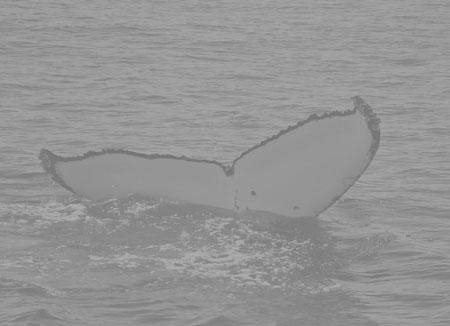
\includegraphics[height=40mm]{1.jpg}}&
%\frame{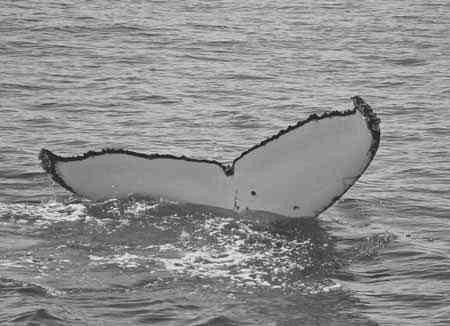
\includegraphics[height=40mm]{1-p.jpg}} \\ 
\vspace{0.2cm}
{
\(
\left[ \begin{array}{ccc}
-1 & 0 & +1 \\
-2 & 0 & +2 \\
-1 & 0 & +1 \end{array} \right]
\)} 
\hspace{1cm}
& 
{\(
\left[ \begin{array}{ccc}
-1 & -2 & -1 \\
0 & 0 & 0 \\
+1 & +2 & +1 \end{array} \right]
\)} \\
\small \textbf{ \( G_x \) } 
\hspace{1cm}
&
\small \textbf{ \( G_y \) } 
\end{tabular}
\end{center}

برای یافتن لبه‌ها، لازم است هر یک از فیلترهای بالا را بر تصویر اعمال کنیم (همگشت یا \lr{Convolution} کنیم) و سپس تصاویر حاصل را با هم جمع کنیم. نتایج اعمال آن بر دو تصویر در زیر آمده‌است. 
در این پیاده‌سازی، توسط تابع 
\lr{filter2D}
، هر کدام از فیلتر‌های بالا را اعمال نمودیم و نتایج حاصل را، با استفاده از تابع 
\lr{addWeighted}
، با وزن‌های یکسان \( 0.5 \) ، جمع نمودیم.

برای تصویر خانه، نتایج اعمال سوبل در هر یک از راستاهای عمودی و افقی نیز آورده شده‌است.

\begin{center}
\begin{tabular}{@{}cc@{}}
\frame{
\includegraphics[height=65mm]{5.jpg}}&
\frame{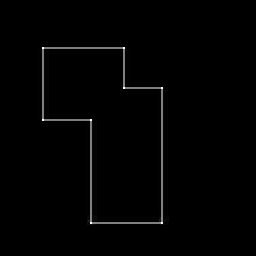
\includegraphics[height=65mm]{5-edgeSobel.png}} \\ 
\small \textbf{تصویر اصلی} & \small \textbf{اعمال \lr{Sobel}}
\end{tabular}
\vspace{1cm}
\end{center}

\begin{center}
\makebox[\textwidth]{%
\begin{tabular}{@{}cc@{}}
\frame{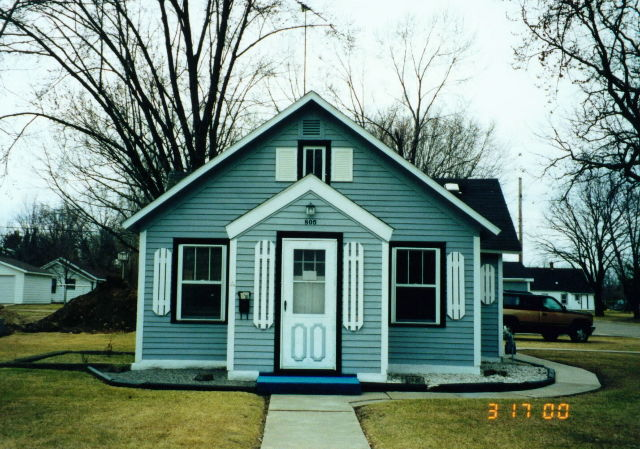
\includegraphics[height=65mm]{332.jpg}}&
\frame{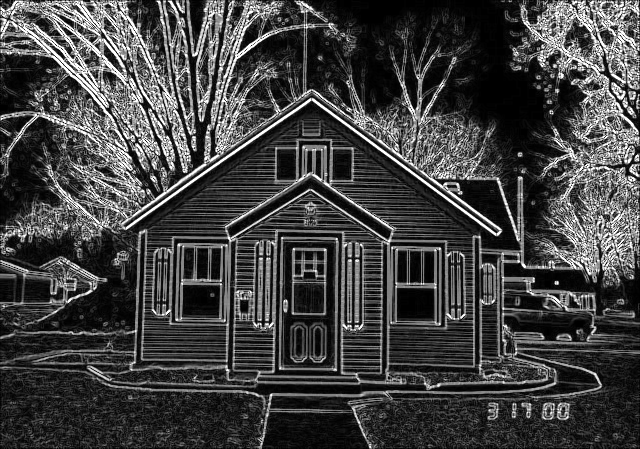
\includegraphics[height=65mm]{332-edgeSobel.png}} \\ 
\small \textbf{تصویر اصلی} & \small \textbf{اعمال سوبل}
\end{tabular}}
\vspace{0.2cm}
\end{center}
 
\vspace{0.2cm}
\begin{center}
\makebox[\textwidth]{%
\begin{tabular}{@{}cc@{}}
\frame{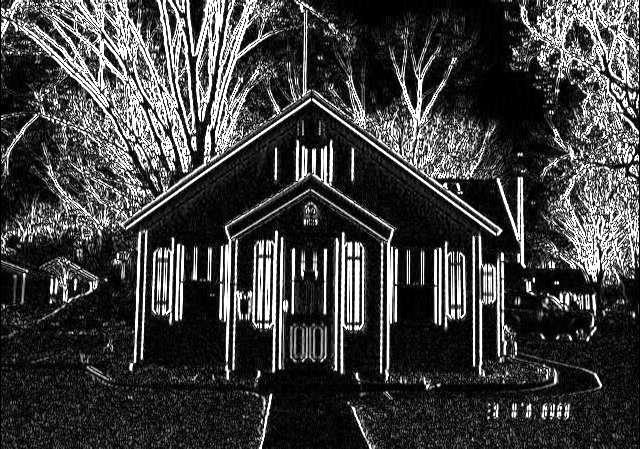
\includegraphics[height=65mm]{332-sobelX.png}}&
\frame{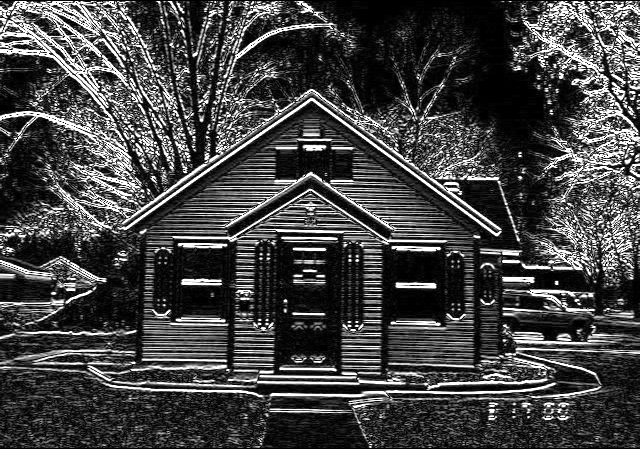
\includegraphics[height=65mm]{332-sobelY.png}} \\ 
\small \textbf{سوبل در راستای \lr{x}} & \small \textbf{سوبل در راستای \lr{y}}
\end{tabular}}
\vspace{0.5cm}
\end{center}

در روش نواتیا ببو، همان‌گونه که در صورت تمرین آمده‌است، از شش فیلتر در زوایای مختلف صفر، ۳۰، ۶۰، ۹۰، ۱۲۰ و ۱۵۰ درجه، استفاده شده‌است. این باعث می‌شود تا گوشه‌های جهت‌داری که از دید سوبل پنهان می‌ماند یا تضعیف می‌شد نیز به خوبی مشخص باشد.
ایراد این روش، آن است که باید پس از اعمال فیلتر، یک عمل 
\lr{Thresholding}
(آستانه‌ای کردن) انجام شود و در صورت نیاز، نازک‌سازی نیز لازم است. در ادامه نمونه‌ای از اعمال این فیلترها آورده شده‌است. نتایج اعمال هر شش فیلتر، با وزن‌های مساوی با هم جمع شده‌اند. 

\begin{center}
\makebox[\textwidth]{%
\begin{tabular}{@{}cc@{}}
\frame{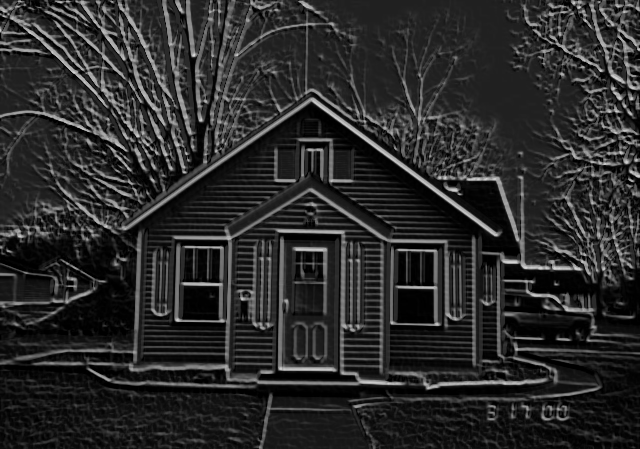
\includegraphics[height=65mm]{332-babu-0.png}}&
\frame{
\includegraphics[height=65mm]{5-babu-0.png}}
\\ 
\small \textbf{اعمال فیلتر‌های نواتیا ببو} &
\small \textbf{اعمال فیلتر‌های نواتیا ببو}  \small 
\end{tabular}}
\vspace{0.2cm}
\end{center}

از دیگر معایب نواتیا ببو، کند بودن آن به دلیل زیاد بودن عملیات آن است.
از طرفی، فیلتر سوبل، در عین سریع‌بودن و عدم نیاز به عملیات اضافی، لبه‌های جهت‌دار ضعیف را از دست می‌دهد.

\subsection{\lr{Canny}}

\textbf{پرسش: }
به طور خلاصه توضیح دهید لبه‌یاب کنی چگونه عمل می‌کند. هدف از کرنل گوسی در این لبه‌یاب چیست؟ این لبه‌یاب را بر تصویر شماره ۴ اعمال کنید.


\textbf{پاسخ: } 
این لبه‌یاب که به لبه‌یاب بهینه نیز معروف است،‌ سه ویژگی اصلی دارد: 

\begin{itemize}
\renewcommand{\labelitemi}{$\bullet$}
\item \textbf{خطای کم:‌ } 
فقط لبه‌های موجود را به خوبی تشخیص می‌دهد.
\item \textbf{مکان‌یابی خوب: } 
فاصله‌ی لبه‌ی تشخیص‌ داده‌شده تا لبه‌ی واقعی در تصویر، کمینه است.
\item \textbf{واکنش کمینه: } 
به هر لبه فقط یک‌بار واکنش نشان می‌دهد.
\end{itemize}

نحوه کار این لبه‌یاب، به این شکل است که ابتدا توسط یک کرنل گاسی، نویز را از تصویر حذف می‌کند.
سپس با استفاده از کرنل سوبل، که در زیر آورده شده‌است، گرادیان شدت روشنایی را حساب می‌کند.

سپس جهت و بزرگی گردایان را از روابط زیر به‌دست می‌آورد.

\vspace{-0.5cm}
\begin{equation}
\label{gradianMag}
G = \sqrt {G_x^2 + G_y^2}
\vspace{0.2cm}
\end{equation}

\begin{equation}
\label{gradianOr}
\theta = arctan ({G_y \over G_x})
\end{equation}
که جهت گرادیان، به یکی از زوایای صفر، ۴۵، ۹۰ و یا ۱۳۵ درجه، گرد می‌شود.
سپس از پیکسل‌هایی که بیشینه‌ی محلی نیستند صرف نظر می‌کند، زیرا احتمال این که این نقاط بر روی لبه باشند، پایین است. 
پس از آن، در مرحله‌ی پایانی، از دو مقدار آستانه برای تشخیص لبه استفاده می‌کند؛ به این ترتیب که اگر در یک پیکسل مقدار گرادیان بیشتر از حد آستانه‌ی بالا باشد، آن پیکسل به عنوان لبه انتخاب می‌شود. اگر مقدار گرادیان از حد آستانه‌ی پایینی کمتر باشد، انتخاب نمی‌شود. و در نهایت، اگر مقدار گرادیان مقداری بین دو حد آستانه باشد، تنها در صورتی انتخاب می‌شود که به یک پیکسل روی لبه (بالاتر از حد آستانه) متصل باشد. 
در این روش، پیشنهاد می‌شود نسبت حد آستانه‌ی بالا به پایین، بین ۲:۱ و ۳:۱ باشد.

همان‌گونه که گفته‌شد، کرنل گاسی برای رفع نویز استفاده می‌شود، چون کرنل سوبل که برای پیدا کردن لبه‌ها استفاده می‌شود، بسیار به نویز حساس است.
در 
\lr{OpenCV} 
برای اعمال این لبه‌یاب، ابتدا با فراخوانی تابع زیر، عمل رفع نویز را با یک کرنل گاسی 
\( 3 \times 3 \) 
انجام می‌دهیم:

\leftline{\lr{blur( src, dst, Size(3,3));}}
سپس تابع زیر را برای اعمال کنی با کرنل 
\( 3 \times 3 \) 
فراخوانی می‌کنیم: 

\leftline{\lr{Canny( dst, edgesCanny, lowThreshold, highThreshold, 3);}} 

در زیر، نتیجه‌ی اعمال این روش بر روی تصویر ۴ آمده‌است. حد آستانه‌ی بالا و پایین تصویر مشخص شده‌است.

\begin{center}
\vspace{5mm}
\begin{tabular}{@{}cc@{}}
\frame{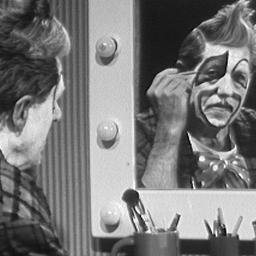
\includegraphics[height=65mm]{4.jpg}} &
\frame{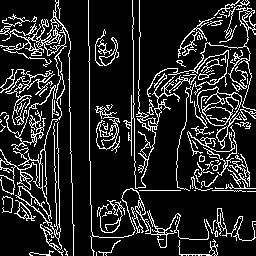
\includegraphics[height=65mm]{4-edgeCanny1-255.png}} \\ 
\small \textbf{تصویر ۴} & \small \textbf{کنی با آستانه‌ی پایین ۱ و آستانه‌ی بالای ۲۵۵}
\end{tabular}
\vspace{0.5cm}
\end{center} 
\vspace{0.2cm}

\vspace{0.5cm}
\subsection{پارامترهای \lr{Canny}‬}

\textbf{پرسش: }
لبه‌یاب کنی سه پارامتر دارد، تغییر مقدار این پارامتر‌ها چه تاثیری بر نتیجه‌ی حاصله دارد؟ اندازه‌ی کرنل ۳، ۵ و ۷ را بر تصویری دل‌خواه اعمال کرده و نتیجه را مقایسه کنید. اگر آستانه‌ی بالا را از ۲۵۵ به ۱۲۸ تغییر دهیم چه تغییری بر تصویر نهایی ایجاد می‌شود؟ نتیجه‌ی تغییر آستانه‌ی پایین از ۱ به ۲۲۰ چیست؟
 
\textbf{پاسخ: }

\begin{itemize}
\renewcommand{\labelitemi}{$\bullet$}
\item \textbf{حد آستانه‌ی پایین:‌ } 
هر اندازه کمتر باشد، لبه‌های ضعیف‌تر کم‌تری حذف می‌شوند و لبه‌های ضعیف بیشتری، برای بررسی بعدی انتخاب می‌شوند. زیاد کردن این مقدار نیز باعث شکسته‌تر شدن لبه‌های یافت‌شده می‌شود.
\item \textbf{حد آستانه‌ی بالا: } 
هر اندازه بیشتر باشد، تنها لبه‌های قوی‌تر انتخاب خواهند شد. 
\item \textbf{اندازه کرنل: } 
از آنجا که کرنل بزرگ‌تر، گرادیان را با توجه به محدوده‌ی وسیع‌تری محاسبه می‌کند، از دقت بیشتری برخوردار است.
\end{itemize}
نتیجه‌ی لبه‌یابی و اعمال تغییرات بر روی عکس خانه در بخش قبلی، در زیر آورده شده‌است.

\vspace{0.2cm}
\begin{center}
\makebox[\textwidth]{%
\begin{tabular}{@{}cc@{}}
\frame{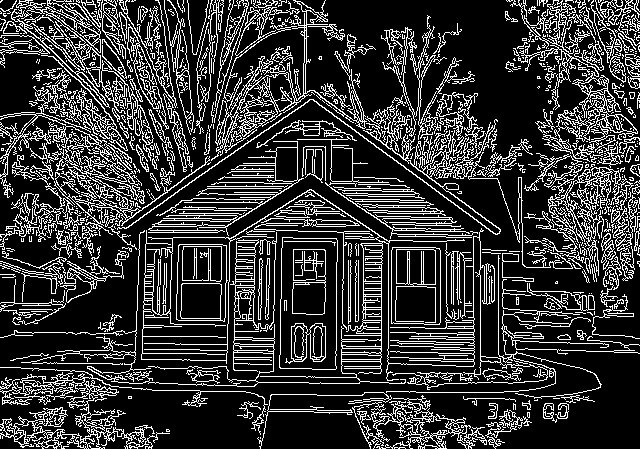
\includegraphics[height=65mm]{332-edgeCanny1-255-k3.png}} &
\frame{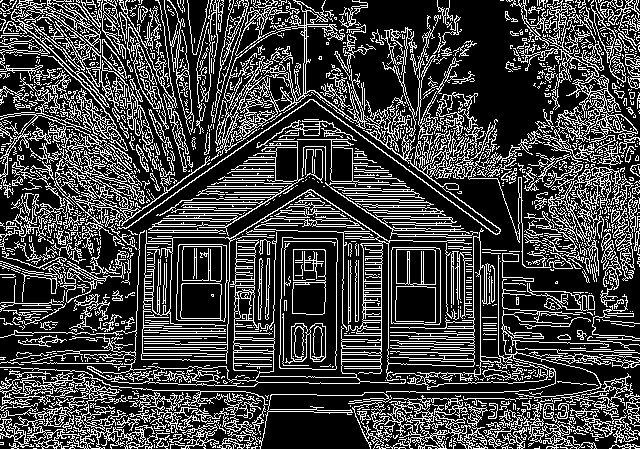
\includegraphics[height=65mm]{332-edgeCanny1-128-k3.png}} \\ 
\small \textbf{کنی ۱-۲۵۵ با کرنل ۳} & 
\small \textbf{کنی ۱-۱۲۸ با کرنل ۳}
\end{tabular}}
\end{center}

\vspace{0.2cm}
\begin{center}
\makebox[\textwidth]{%
\begin{tabular}{@{}cc@{}}
\frame{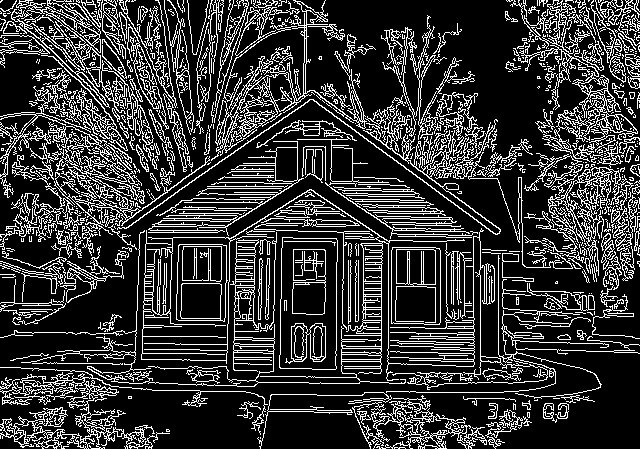
\includegraphics[height=65mm]{332-edgeCanny1-255-k3.png}} &
\frame{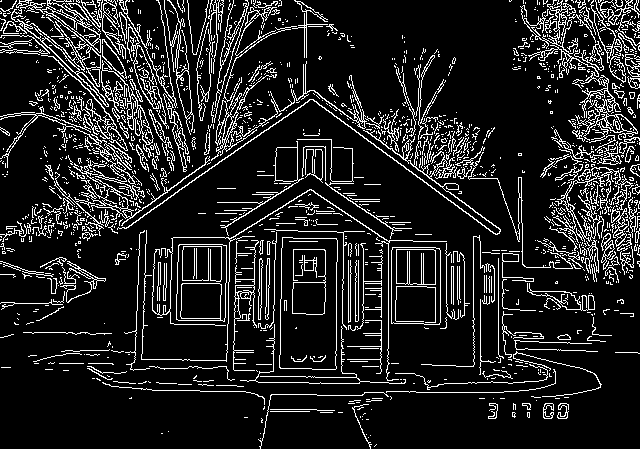
\includegraphics[height=65mm]{332-edgeCanny220-255-k3.png}} \\ 
\small \textbf{کنی ۱-۲۵۵ با کرنل ۳} & 
\small \textbf{کنی ۲۲۰-۲۵۵ با کرنل ۳}
\end{tabular}}
\end{center}
همان‌گونه که مشاهده می‌کنید، با کاهش حد آستانه‌ی بالا به ۱۲۸، لبه‌های ضعیف‌تر بیشتری یافت شده‌اند. تشخیص تمامی برگ‌ها و چمن‌ها حاصل این کاهش است.
همچنین با افزایش حد آستانه‌ی پایین، لبه‌های ضعیف مانند چمن‌ها حذف شده‌اند و لبه‌های قوی مانند پیرامون خانه و ساعت در گوشه‌ی پایین تصویر، بیشتر به چشم می‌آیند.

نتیجه‌ی تغییرات اندازه کرنل نیز آورده شده‌است. مشاهده می‌کنید که با افزایش اندازه، دقت بیشتر شده‌است. 

\vspace{0.2cm}
\begin{center}
\makebox[\textwidth]{%
\begin{tabular}{@{}cc@{}}
\frame{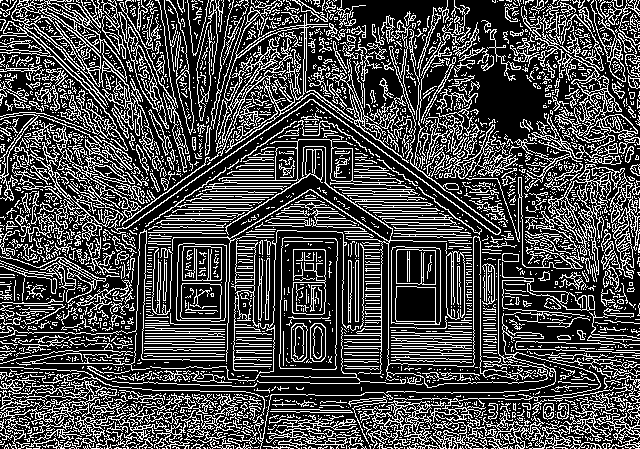
\includegraphics[height=65mm]{332-edgeCanny1-255-k5.png}} &
\frame{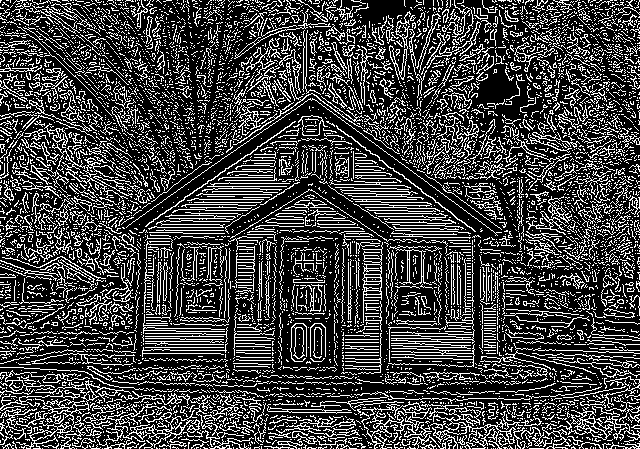
\includegraphics[height=65mm]{332-edgeCanny1-255-k7.png}} \\ 
\small \textbf{کنی ۱-۲۵۵ با کرنل ۵} & 
\small \textbf{کنی ۱-۲۵۵ با کرنل ۷}
\end{tabular}}
\end{center}

\vspace{0.5cm}
\subsection{مقایسه کنی و لبه‌یاب‌های کلاسیک}
\textbf{پرسش: }
لبه‌یاب کنی نسبت به لبه‌یاب‌های کلاسیک (مثل سوبل و نواتیا ببو) چه مزایا و معایبی دارد؟ نتیجه این دو روش را مقایسه کنید.

\textbf{پاسخ: }
در استفاده‌ از کنی، پیدا کردن مقادیر آستانه‌‌ای مناسب برای هر تصویر متفاوت و زمان‌بر است. همچنین اجرای خود الگوریتم از لبه‌یاب‌های کلاسیک زمان‌برتر است. با این حال لبه‌های یافت‌شده توسط کنی از دقت و بهینگی بیشتری برخوردار هستند و نازک‌سازی اضافی نیز نیاز نیست. دلایل بهینگی در بخش ۲.۱ آورده‌شد. 
از طرفی لبه‌یاب‌های کلاسیک، ممکن است لبه‌های مجزای بهتری به دست دهند که با مقایسه‌ی دو عکس زیر در خصوص چمن‌های تشخیص داده‌شده به این نتیجه می‌رسیم. چرا که کنی، ممکن است لبه‌های ضعیف متصل به لبه‌های قوی را، بر روی یک لبه‌ی قوی تشخیص دهد، حال آن‌که در سوبل چنین نیست و لبه‌ها از بزرگی و جهت مستقل از یک‌دیگر برخوردار هستند.
همچنین احتمال شکستگی لبه‌ها در کنی وجود دارد ولی در سوبل و نواتیا ببو این چنین نیست.

\vspace{0.2cm}
\begin{center}
\makebox[\textwidth]{%
\begin{tabular}{@{}cc@{}}
\frame{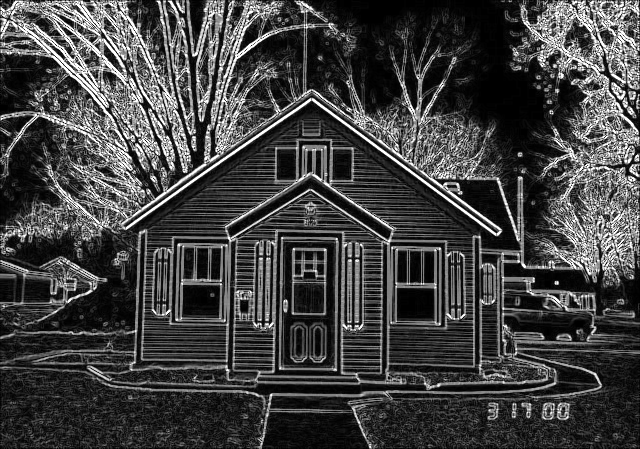
\includegraphics[height=65mm]{332-edgeSobel.png}} &
\frame{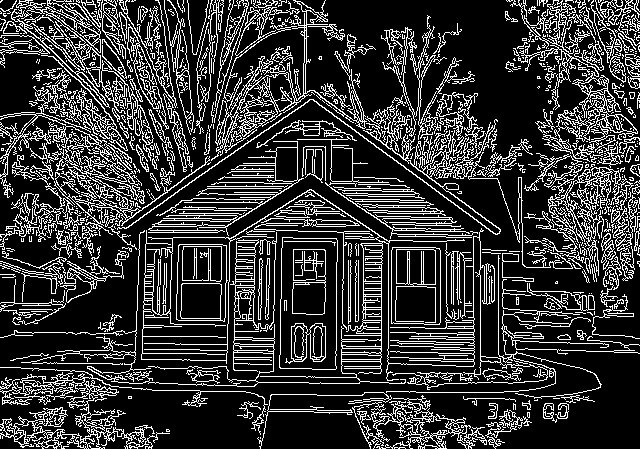
\includegraphics[height=65mm]{332-edgeCanny1-255-k3.png}} \\ 
\small \textbf{اعمال سوبل} & 
\small \textbf{کنی ۱-۲۵۵ با کرنل ۳}
\end{tabular}}
\vspace{0.5cm}
\end{center}

\vspace{0.5cm}
\section{ بخش دوم: تبدیل هاف} 
\vspace{0.5cm}
\subsection{تبدیل هاف برای تشخیص خط}

\textbf{پرسش: }
 یکی از روش‌های تشخیص خط، استفاده از تبدیل هاف است. معمولا ورودی تبدیل هاف چیست؟ تبدیل هاف را بر تصویری شامل خطوط اعمال کرده و خطوط بدست آمده را رسم کنید.

\textbf{پاسخ: }
از آن‌جا که تبدیل هاف، نیاز دارد نقاط موجود در عکس را برای تشخیص خط، به فضای پارامتری ببرد، بنابراین تنها نقاط موجود در ورودی هاف باید نقاطی باشند که ممکن است بر روی خطی قرار داشته‌باشند. با این فرض، ورودی تبدیل هاف باید لبه‌های موجود در عکس باشد تا در صورت وجود لبه‌ای به صورت خط صاف، تشخیص داده‌شود. 
در زیر نتیجه‌ی اعمال هاف با استفاده از تابع 
\lr{HoughLines}
آورده شده‌است.

\vspace{0.2cm}
\begin{center}
\makebox[\textwidth]{%
\begin{tabular}{@{}cc@{}}
\frame{
\includegraphics[height=65mm]{111.jpg}} &
\frame{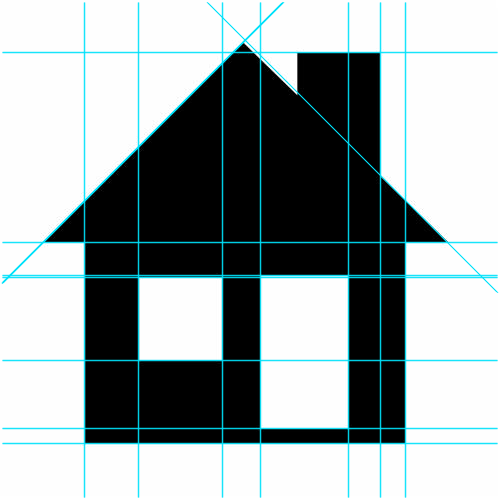
\includegraphics[height=65mm]{111-houghLines.png}} \\ 
\small \textbf{تصویر اصلی} & 
\small \textbf{هاف: \lr{\( \theta = 1^{\circ}, r=0.1, threshold=50\)}}
\end{tabular}}
\end{center}

\vspace{0.5cm}
\subsection{اثر نویز بر هاف}

\textbf{پرسش: }
نویز چه تاثیری بر تبدیل هاف دارد؟ برای بررسی این سوال، به تصویر حاصله از لبه‌یاب، نویز گوسی اضافه کرده و تبدیل هاف را اعمال کنید. تبدیل هاف تا چه واریانسی از نویز گوسی را می‌تواند تحمل کند و خطوط را تشخیص دهد؟ (تصویر شماره ۵)

\textbf{پاسخ: }
نویز سبب می‌شود هاف نقاطی با فواصل زیاد که در تصویر اصلی روی یک خط نیستند ولی در نویز خام اضافه‌شده، روی یک خط هستند را تاثیر دهد و خطوط اضافه‌ی بسیاری را پیدا کند. در ادامه چند نمونه آورده شده‌است که مشاهده می‌کنیم با میانگین ۳۰۰ برای نویز گاسی، نتیجه‌ی هاف از واریانس ۷۰ به بالا غیر قابل قبول است.

\vspace{0.2cm}
\begin{center}
\makebox[\textwidth]{%
\begin{tabular}{@{}cc@{}}
\frame{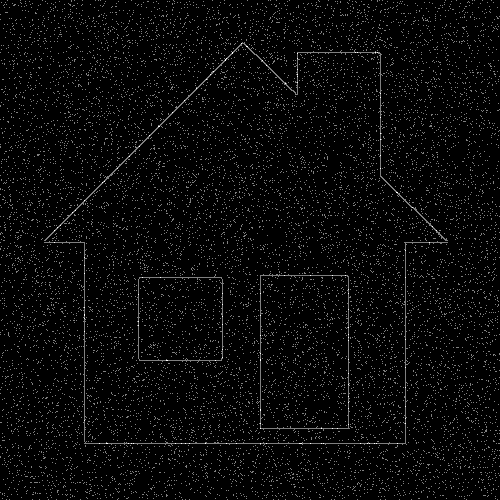
\includegraphics[height=65mm]{111-houghInp-Sig63.png}} &
\frame{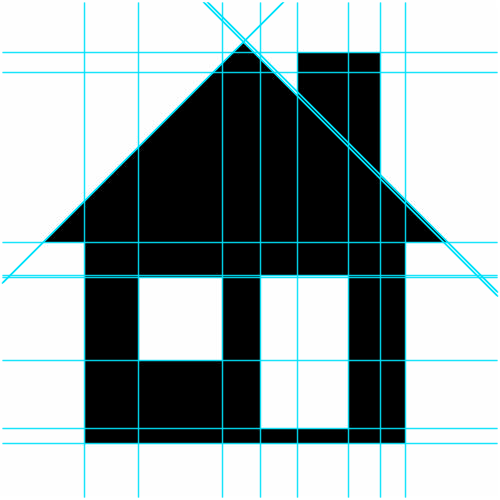
\includegraphics[height=65mm]{111-houghLines-Sig63.png}} \\ 
\small \textbf{تصویر ورودی \lr{\( \sigma = 63\)} } & 
\small \textbf{هاف: \lr{\( \theta = 1^{\circ}, r=0.1, threshold=50\)}}
\end{tabular}}
\end{center}


\vspace{0.2cm}
\begin{center}
\makebox[\textwidth]{%
\begin{tabular}{@{}cc@{}}
\frame{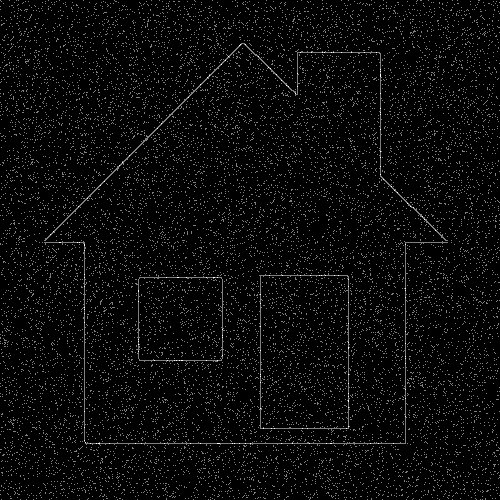
\includegraphics[height=65mm]{111-houghInp-Sig67.png}} &
\frame{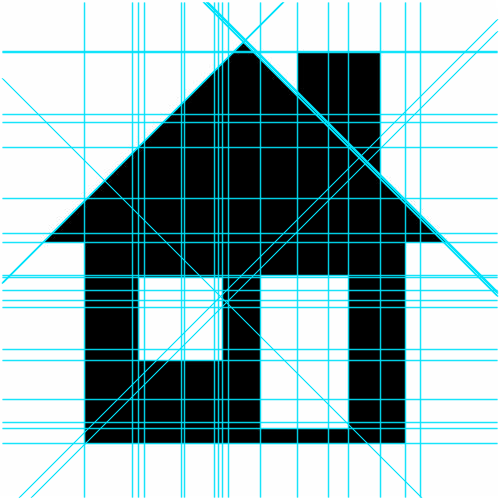
\includegraphics[height=65mm]{111-houghLines-Sig67.png}} \\ 
\small \textbf{تصویر ورودی \lr{\( \sigma = 67\)} } & 
\small \textbf{هاف: \lr{\( \theta = 1^{\circ}, r=0.1, threshold=50\)}}
\end{tabular}}
\end{center}


\vspace{0.2cm}
\begin{center}
\makebox[\textwidth]{%
\begin{tabular}{@{}cc@{}}
\frame{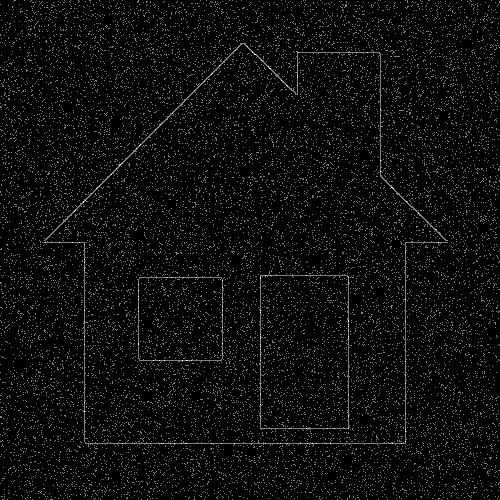
\includegraphics[height=65mm]{111-houghInp-Sig69.png}} &
\frame{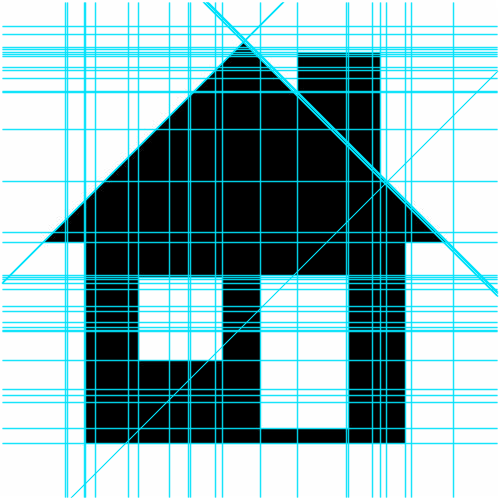
\includegraphics[height=65mm]{111-houghLines-Sig69.png}} \\ 
\small \textbf{تصویر ورودی \lr{\( \sigma = 69\)} } & 
\small \textbf{هاف: \lr{\( \theta = 1^{\circ}, r=0.1, threshold=50\)}}
\end{tabular}}
\end{center}


\vspace{0.2cm}
\begin{center}
\makebox[\textwidth]{%
\begin{tabular}{@{}cc@{}}
\frame{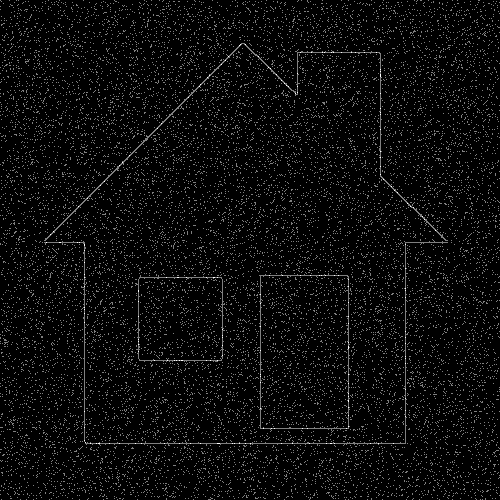
\includegraphics[height=65mm]{111-houghInp-Sig70.png}} &
\frame{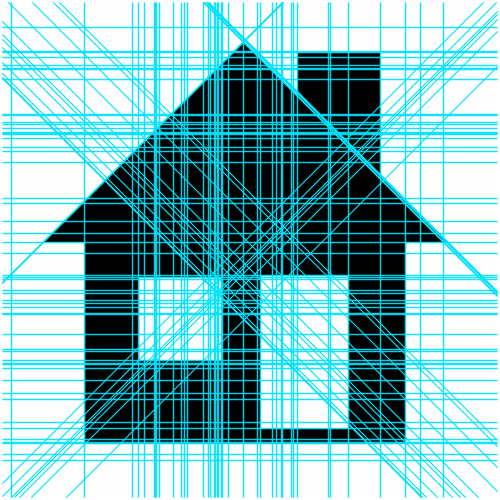
\includegraphics[height=65mm]{111-houghLines-Sig70.png}} \\ 
\small \textbf{تصویر ورودی \lr{\( \sigma = 70\)} } & 
\small \textbf{هاف: \lr{\( \theta = 1^{\circ}, r=0.1, threshold=50\)}}
\end{tabular}}
\end{center}


\vspace{0.2cm}
\begin{center}
\makebox[\textwidth]{%
\begin{tabular}{@{}cc@{}}
\frame{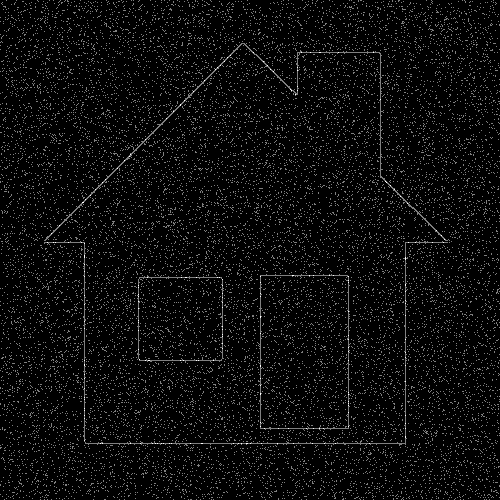
\includegraphics[height=65mm]{111-houghInp-Sig71.png}} &
\frame{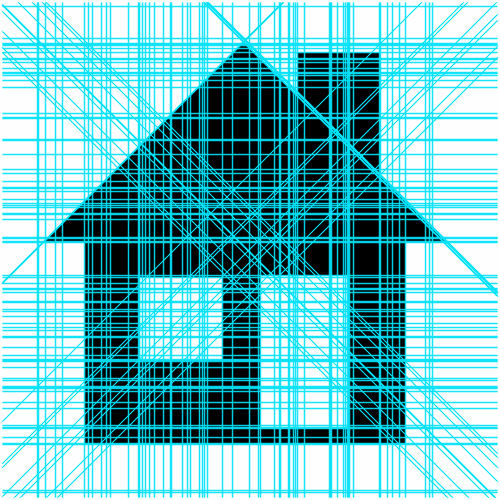
\includegraphics[height=65mm]{111-houghLines-Sig71.png}} \\ 
\small \textbf{تصویر ورودی \lr{\( \sigma = 71\)} } & 
\small \textbf{هاف: \lr{\( \theta = 1^{\circ}, r=0.1, threshold=50\)}}
\end{tabular}}
\end{center}


\vspace{0.2cm}
\begin{center}
\makebox[\textwidth]{%
\begin{tabular}{@{}cc@{}}
\frame{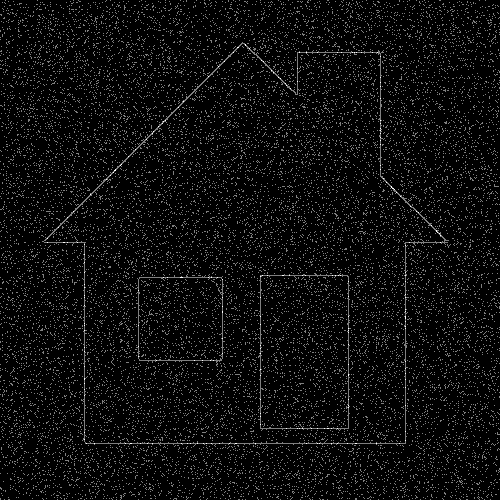
\includegraphics[height=65mm]{111-houghInp-Sig75.png}} &
\frame{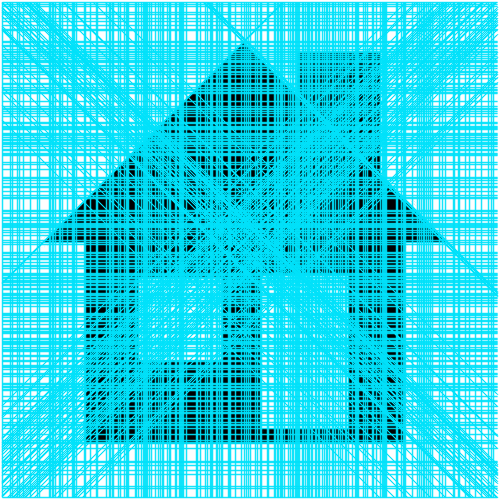
\includegraphics[height=65mm]{111-houghLines-Sig75.png}} \\ 
\small \textbf{تصویر ورودی \lr{\( \sigma = 75\)} } & 
\small \textbf{هاف: \lr{\( \theta = 1^{\circ}, r=0.1, threshold=50\)}}
\end{tabular}}
\end{center}

\vspace{0.5cm}
\subsection{هاف دایره}

\textbf{پرسش: }
 تبدیل دایره هاف را بر تصویری شامل اشکال دایره‌ای اعمال کرده و پارامترهای آن را به گونه‌ای تنظیم کنید که دایره‌ها را بیابد.
 
\textbf{پاسخ: }

با اعمال فیلتر گاسی رفع نویز با مقادیر پارامترهای زیر: 

\leftline{\lr{GaussianBlur(img, img, Size(5, 5), 1,1 );}}

و هاف دایره با پارامترهای زیر: 

\leftline{\lr{HoughCircles(img, circles, CV\_HOUGH\_GRADIENT, 0.1,} }
\lr{img.rows/20, 100, 39, 1,100 );}

دایره‌های موجود در تصویر زیر را پیدا کردیم. 

\vspace{0.2cm}
\begin{center}
\makebox[\textwidth]{%
\begin{tabular}{@{}cc@{}}
\frame{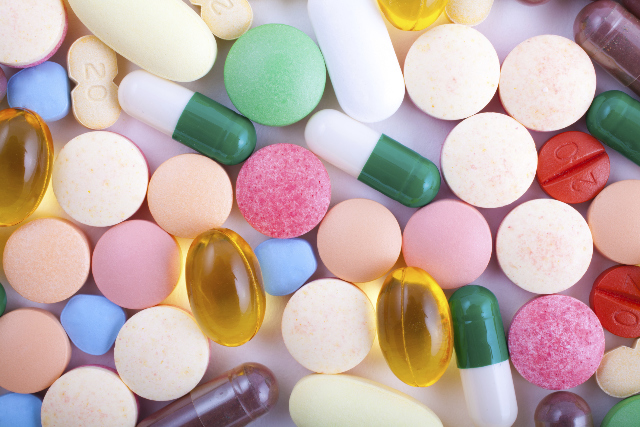
\includegraphics[height=65mm]{pills.jpg}} &
\frame{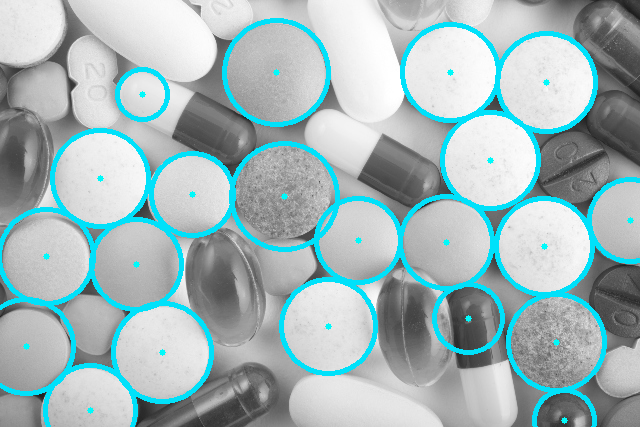
\includegraphics[height=65mm]{pills-hoghCirc.png}} \\ 
\small \textbf{تصویر ورودی} & 
\small \textbf{هاف دایره}
\end{tabular}}
\end{center}

\vspace{0.5cm}
\section{بخش سوم: کانتورها}
\vspace{0.5cm}
\subsection{کانتور}

\textbf{پرسش: }
کانتور چیست؟ در 
\lr{OpenCV}
چه توابعی برای پیدا کردن کانتور و یافتن خصوصیات آن تعریف شده است؟ به طور خلاصه توضیح دهید. 
 
\textbf{پاسخ: }

به طور کلی، کانتور یک منحنی روی یک تابع دو متغیره است که تابع در روی این منحنی، مقادیر یکسانی دارد. حال در تصویر، به هر منحنی که روی آن، پیکسل‌ها یک خاصیت را داشته‌باشند (نظیر رنگ، شدت روشنایی و یا گرادیان)، یک کانتور می‌گویند.
از خصوصیات کانتورها که در 
\lr{OpenCV}
به‌دست می‌آید می‌توان به تعداد آن‌ها، سلسله‌مراتب یا ترتیب آن‌ها، فرزندان و والدین هر کانتور و نیز کانتورهای هم‌سطح آن، اشاره کرد. 
\vspace{0.5cm}
\subsection{\lr{findContours}}

\textbf{پرسش: }
تابع 
\lr{findContours}
از چه روشی برای تعیین پیرامون استفاده می‌کند؟ پارامتر‌های این تابع چیست؟ این تابع را بر روی یک تصویر اعمال کرده و نتیجه را نشان دهید.
 
\textbf{پاسخ: }
با استفاده از خروجی لبه‌یاب کنی، از روش‌های زیر استفاده می‌کند:

\lr{CV\_CHAIN\_APPROX\_NONE}
 : در این روش هر همسایگی پیکسل برای وجود برروی کانتور بررسی می‌شود.

\lr{CV\_CHAIN\_APPROX\_SIMPLE}
 : در راستای عمودی، افقی و قطری، پیکسل‌های روی یک قطعه را فشرده می‌کند و تنها نقاط انتهایی را باقی می‌گذارد.

روش مورد استفاده، در پارامترهای ورودی تابع، داده می‌شود.
پارامتر مهم دیگر این تابع، 
\lr{mode}
می‌باشد که تعیین‌کننده‌ی چگونگی محاسبه‌ی کانتورهاست. برای نمونه، فقط کانتورهای بیرونی محاسبه شوند یا همه‌ی کانتورها.
نتیجه‌ی اعمال این تابع را در تصویر زیر مشاهده می‌فرمایید که در آن کانتورها با رنگ‌های متفاوت نمایش داده‌ شده‌اند. به آسانی متوجه خواهید شد در دو قرص صورتی‌رنگ و در کپسول تیره‌رنگ پایین صفحه، نواحی مشابه تصویر، در یک کانتور آمده‌اند. دقت شود که این کانتورها، با توجه به خروجی لبه‌یاب کنی محاسبه شده‌اند.
این عمل، خود به نوعی تقطیع تصویر مبتنی بر لبه‌ می‌باشد.

\vspace{0.2cm}
\begin{center}
\makebox[\textwidth]{%
\begin{tabular}{@{}cc@{}}
\frame{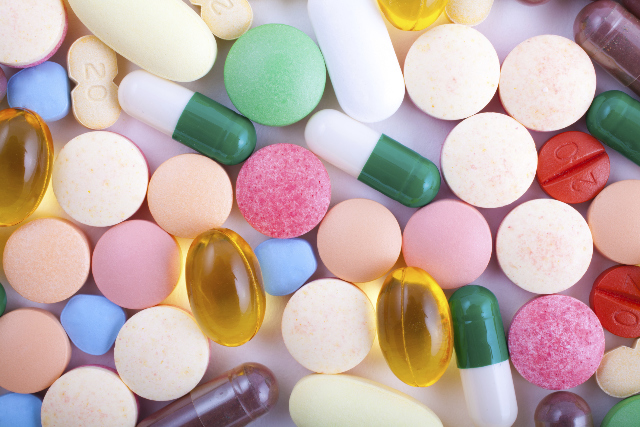
\includegraphics[height=65mm]{pills.jpg}} &
\frame{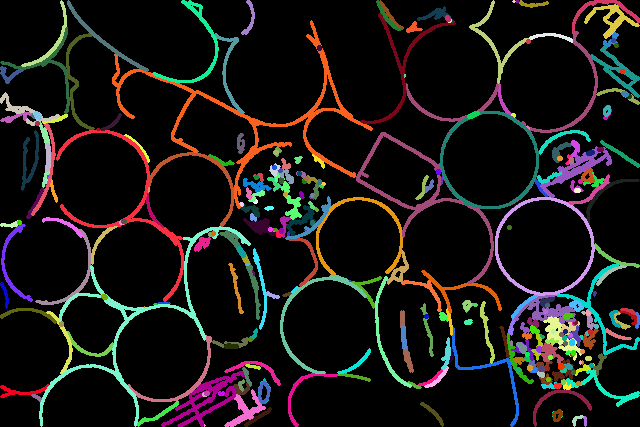
\includegraphics[height=65mm]{pills-contours.png}} \\ 
\small \textbf{تصویر ورودی} & 
\small \textbf{کانتورها}
\end{tabular}}
\vspace{0.6cm}
\end{center}

\newpage
تصویری از محیط نرم‌افزار طراحی‌شده: 
\LTRfootnote{\vspace{0.2cm} Based on Qt 5.2.1 (GCC 4.8.2 20140206 (prerelease), 64 bit) - C++11 }

\vspace{0.2cm}
\begin{center}
\makebox[\textwidth]{%
\begin{tabular}{@{}cc@{}}
\frame{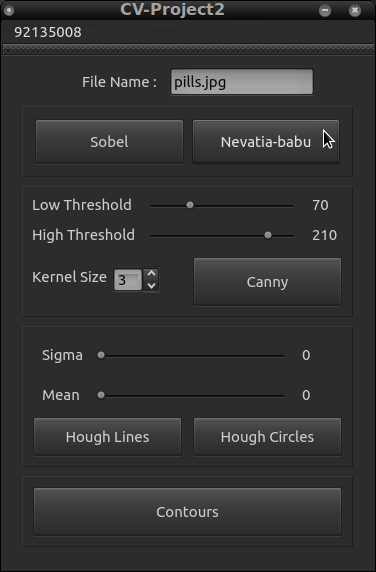
\includegraphics[width=80mm]{vision2.png}} &
\\ 
\end{tabular}}
\end{center}


\end{document} 
